\documentclass[
	12pt,				
	openright,		
	twoside,	
	a4paper,
	english,	
	brazil	
	]{abntex2}
\usepackage{lmodern}		
\usepackage[T1]{fontenc}	
\usepackage[utf8]{inputenc}
\usepackage{lastpage}	
\usepackage{indentfirst}
\usepackage{color}	
\usepackage{graphicx}
\usepackage{microtype}
\graphicspath{{./imagens/}}
\usepackage{lipsum}			
\usepackage[brazilian,hyperpageref]{backref}	 
\usepackage[alf]{abntex2cite}	
\renewcommand{\backrefpagesname}{Citado na(s) página(s):~}
\renewcommand{\backref}{}
\renewcommand*{\backrefalt}[4]{
	\ifcase #1 %
		Nenhuma citação no texto.%
	\or
		Citado na página #2.%
	\else
		Citado #1 vezes nas páginas #2.%
	\fi}%
\titulo{Análise de Sistemas de Detecção de Intrusão}
\autor{Glenon Mateus Barbosa Araújo}
\local{Brasil}
\data{\the\year}
\orientador{Dr. Roberto Samarone dos Santos Araújo}
%\coorientador{}
\instituicao{
  Universidade Federal do Pará -- UFPA
  \par
  Faculdade de Computação
  \par
  Bacharelado em Ciência da Computação}
\tipotrabalho{Trabalho de Conclusão de Curso}
\preambulo{Trabalho de Conclusão de Curso submetida a graduação em Ciência da Computação da UFPA}
\definecolor{blue}{RGB}{41,5,195}
\makeatletter
\hypersetup{
     	%pagebackref=true,
		pdftitle={\@title}, 
		pdfauthor={\@author},
    	pdfsubject={\imprimirpreambulo},
	    pdfcreator={LaTeX with abnTeX2},
		pdfkeywords={abnt}{latex}{abntex}{abntex2}{trabalho acadêmico}, 
		colorlinks=true,       	
    	linkcolor=blue,          
    	citecolor=blue,        	
    	filecolor=magenta,     
		urlcolor=blue,
		bookmarksdepth=4
}
\makeatother
\setlength{\parindent}{1.3cm}
\setlength{\parskip}{0.2cm} 
\makeindex
\begin{document}
\selectlanguage{brazil}
\frenchspacing 
\imprimircapa
\imprimirfolhaderosto*
\begin{fichacatalografica}
	\sffamily
	\vspace*{\fill}
	\begin{center}
	\fbox{\begin{minipage}[c][8cm]{13.5cm}	
	\small
	\imprimirautor
	\hspace{0.5cm} \imprimirtitulo  / \imprimirautor. --
	\imprimirlocal, \imprimirdata-
	\hspace{0.5cm} \pageref{LastPage} p. : il. (algumas color.) ; 30 cm.\\
	\hspace{0.5cm} \imprimirorientadorRotulo~\imprimirorientador\\
	\hspace{0.5cm}
	\parbox[t]{\textwidth}{\imprimirtipotrabalho~--~\imprimirinstituicao,
	\imprimirdata.}\\
	\hspace{0.5cm}
		1. Suricata.
		2. Snort.
		3. IDPS.
		I. Orientador.
		II. Universidade Federal do Pará.
		III. Faculdade de Computação.
		IV. Análise de IDPSs
	\end{minipage}}
	\end{center}
\end{fichacatalografica}
\begin{errata}
Elemento opcional da \citeonline[4.2.1.2]{NBR14724:2011}. Exemplo:
\vspace{\onelineskip}
FERRIGNO, C. R. A. \textbf{Tratamento de neoplasias ósseas apendiculares com
reimplantação de enxerto ósseo autólogo autoclavado associado ao plasma
rico em plaquetas}: estudo crítico na cirurgia de preservação de membro em
cães. 2011. 128 f. Tese (Livre-Docência) - Faculdade de Medicina Veterinária e
Zootecnia, Universidade de São Paulo, São Paulo, 2011.
\begin{table}[htb]
\center
\footnotesize
\begin{tabular}{|p{1.4cm}|p{1cm}|p{3cm}|p{3cm}|}
  \hline
   \textbf{Folha} & \textbf{Linha}  & \textbf{Onde se lê}  & \textbf{Leia-se}  \\
    \hline
    1 & 10 & auto-conclavo & autoconclavo\\
   \hline
\end{tabular}
\end{table}
\end{errata}
\begin{folhadeaprovacao}
  \begin{center}
    {\ABNTEXchapterfont\large\imprimirautor}
    \vspace*{\fill}\vspace*{\fill}
    \begin{center}
      \ABNTEXchapterfont\bfseries\Large\imprimirtitulo
    \end{center}
    \vspace*{\fill}
    
    \hspace{.45\textwidth}
    \begin{minipage}{.5\textwidth}
        \imprimirpreambulo
    \end{minipage}%
    \vspace*{\fill}
   \end{center}
        
   Trabalho aprovado. \imprimirlocal, 24 de novembro de 2012:
   \assinatura{\textbf{\imprimirorientador} \\ Orientador} 
   %\assinatura{\textbf{Professor} \\ Convidado 1}
   %\assinatura{\textbf{Professor} \\ Convidado 2}
   %\assinatura{\textbf{Professor} \\ Convidado 3}
   %\assinatura{\textbf{Professor} \\ Convidado 4}
      
   \begin{center}
    \vspace*{0.5cm}
    {\large\imprimirlocal}
    \par
    {\large\imprimirdata}
    \vspace*{1cm}
  \end{center}
  
\end{folhadeaprovacao}
\begin{dedicatoria}
   \vspace*{\fill}
   \centering
   \noindent
   \textit{•} \vspace*{\fill}
\end{dedicatoria}
\begin{agradecimentos}
\end{agradecimentos}
\begin{epigrafe}
    \vspace*{\fill}
	\begin{flushright}
		\textit{•}
	\end{flushright}
\end{epigrafe}
\setlength{\absparsep}{18pt} 
\begin{resumo}
 \textbf{Palavras-chave}: Segurança, Suricata, Snort, Sistema de Detecção de Intrusão, Sistema de Prevenção de Intrusão, IDS, IPS.
\end{resumo}
\begin{resumo}[Abstract]
 \begin{otherlanguage*}{english}
   \vspace{\onelineskip}
 
   \noindent 
   \textbf{Keywords}: Security, Suricata, Snort, Intrusion Detection System, Intrusion Prevention System, IDS, IPS.
 \end{otherlanguage*}
\end{resumo}
\pdfbookmark[0]{\listfigurename}{lof}
\listoffigures*
\cleardoublepage
\pdfbookmark[0]{\listtablename}{lot}
\listoftables*
\cleardoublepage
\begin{siglas}
  \item[IDS] \textit{Intrusion Detection System}
  \item[IPS] \textit{Intrusion Prevention System}
  \item[SDI] \textit{Sistema de Detecção de Intrusão}
  \item[SPI] \textit{Sistema de Prevenção de Intrusão}
  \item[IDPS] \textit{Intrusion Detection and Prevention System}
  \item[HIDS] \textit{Host Based Intrusion Detection Systems}
  \item[NIDS] \textit{Network Based Intrusion Detection Systems}
  \item[MB] \textit{Megabytes}
  \item[GB] \textit{Gigabytes}
  \item[SO] \textit{Sistema Operacional}
  \item[JSON] \textit{JavaScript Object Notation}
  \item[DoS] \textit{Denial of Service}
  \item[CAIS] \textit{Centro de Atendimento a Incidentes de Segurança}
\end{siglas}
\pdfbookmark[0]{\contentsname}{toc}
\tableofcontents*
\cleardoublepage
\textual
\chapter{Introdução} \label{ch:introdução}
%- Introdução: Texto introdutório do trabalho, motivação, objetivos,
%metodologia, trabalhos relacionados.
%- Adicionar: objetivos
%- Em cada capitulo adicionar um texto introdutório
%- Adicionar o seguinte texto:
%Este capítulo esta organizado da seguinte forma: A próxima seção
%apresenta .... A Seção XY apresenta...
\section{Motivação} \label{sec:motivação}
\section{Objetivos} \label{sec:objetivos}
\section{Metodologia} \label{sec:metodologia}
\section{Trabalhos Relacionados} \label{sec:relacionados}
\chapter{Segurança em Redes de Computadores} \label{ch:segurança}
\section{Definições} \label{sec:definições}

Para entendemos melhor o que é segurança da informação, precisamos conceituar alguns termos que serão detalhados abaixo \cite{esr-gestao}:
\begin{itemize}
 \item \textbf{Incidente de segurança}: qualquer evento oposto a segurança; por exemplo, ataques de negação de serviços (Denial of Service - DoS), roubo de informações, vazamento e obtenção de acesso não autorizado a informações;
 \item \textbf{Ativo}: qualquer coisa que tenha valor para a organização e para seus negócios. Alguns exemplo: banco de dados, softwares, equipamentos (computadores e notebooks), servidores, elementos de redes (roteadores, switches, entre outros), pessoas, processos e serviços;
 \item \textbf{Ameaça}: qualquer evento que explore vulnerabilidades. Causa potencial de um incidente indesejado, que pode resultar em dano para um sistema ou organização;
 \item \textbf{Vulnerabilidade}: qualquer fraqueza que possa ser explorada e comprometer a segurança de sistemas ou informações. Fragilidade de um ativo ou grupo de ativos que pode ser explorada por uma ou mais ameaças. Vulnerabilidades são falhas que permitem o surgimento de deficiências na segurança geral do computador ou da rede. Configurações incorretas no computador ou na segurança também permitem a criação de vulnerabilidades. A partir dessa falha, as ameaças exploram as vulnerabilidades, que, quando concretizadas, resultam em danos para o computador, para a organização ou para os dados pessoais;
 \item \textbf{Risco}: probabilidade de uma ameaça se concretizar;
 \item \textbf{Ataque}: qualquer ação que comprometa a segurança de uma organização;
 \item \textbf{Impacto}: consequência de um evento.
\end{itemize}

Segurança da Informação proteção das informações, sistemas, recursos e demais ativos contra desastres, erros (intencionais ou não) e manipulação não autorizada, objetivando a redução da probabilidade e do impacto de incidentes de segurança.

Segundo a norma ISO/IEC 27002 \cite{isoiec27002}, segurança da informação é a preservação da confidencialidade, da integridade e da disponibilidade da informação; adicionalmente, outras propriedades, tais como autenticidade, responsabilidade, não repúdio e confiabilidade, podem também estar envolvidas.

Dentre vários conhecimentos que um profissional de segurança deve possuir, o conceito mais básico e considerado o pilar de toda a área de segurança corresponde à sigla CID (Confidencialidade, Integridade e Disponibilidade), de modo que um incidente de segurança é caracterizado quando uma dessas áreas é afetada \cite{seg-redes-sistemas}. Abaixo será detalhado cada item.

\begin{itemize}
 \item \textbf{Confidencialidade}: termo ligado à privacidade de um ativo ou recurso, que deve ser acessível somente por pessoas ou grupos autorizados;
 \item \textbf{Integridade}: possui duas definições, a primeira está relacionada com o fato da informação ter valor correto, a segunda, está ligada à inviolabilidade da informação;
 \item \textbf{Disponibilidade}: está relacionada ao acesso à informação, que deve está disponível quando necessária.
\end{itemize}

Dois dos termos citados são fáceis de ser monitorados pois é perceptível para o usuário: a integridade (identificar se uma informação foi alterada) e a disponibilidade (tentando acessar um serviço e verificando se o mesmo está respondendo adequadamente). No entanto, só é possível identificar se houve quebra da confiabilidade através de auditorias, analisando os registros de acesso (se houver), tornando a identificação complicada e em muitos casos impossível \cite{seg-redes-sistemas}.

Além dos conceito listados, a literatura moderna considera mais alguns conceitos auxiliares, temos:

\begin{itemize}
 \item \textbf{Autenticidade}: garantia que uma informação, produto ou documento foi elaborado ou distribuído pelo autor a quem se atribui;
 \item \textbf{Legalidade}: garantia de que ações sejam realizadas em conformidade com os preceitos legais vigentes e que seus produtos tenham validade jurídica;
 \item \textbf{Não repúdio}: conceito bastante utilizado em certificação digital, onde o emissor de uma mensagem não pode negar que a enviou;
 \item \textbf{Privacidade}: habilidade de uma pessoa controlar a exposição e a disponibilidade de informações acerca de si.
\end{itemize}

\section{Cenário Geral} \label{sec:geral}
%apresentar o cenário geral de uma rede conectada a Internet
\section{Pontos de Vulnerabilidade} \label{sec:vulnerabilidade}
%Ex.: Roteador, firewall, clientes e suas aplicações,
\section{Ataques Comuns à Redes de Computadores} \label{sec:ataques}

Nessa seção será descritos os ataques mais comuns à redes e serviços de organizações privadas e públicas, financeiras ou acadêmicas. Para licitar os ataques dessa seção, levou-se em consideração as estatísticas divulgada semestralmente pelo Centro de Atendimento a Incidentes de Segurança (CAIS) (figura \ref{fig:cais}).

\begin{figure}[!htb]
 \centering
 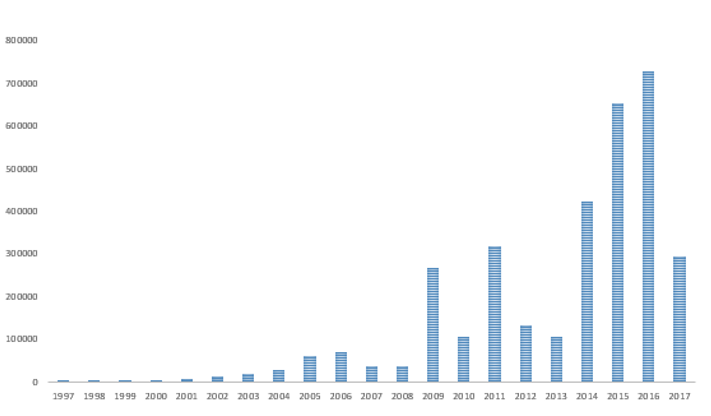
\includegraphics[scale=.5]{incidentes_ano_14.png}
 \caption{Estatísticas de ataques reportadas ao CAIS}
 \label{fig:cais}
\end{figure}

O CAIS é responsável por zela pela segurança da rede Ipê (infraestrutura de rede dedicada à comunidade brasileira de ensino superior), detectando, resolvendo e prevenindo incidentes de segurança. Além disso, tem o papel de orientar (através de publicações de cartilhas) e disseminar boas práticas de segurança da informação, educando e conscientizando usuários de todos os níveis sobre os principais riscos em segurança da informação \cite{cais}.

\subsection{Varredura de Redes} \label{sec:varredura}
\subsection{Exploração de Vulnerabilidades} \label{sec:exploração}
\subsection{Força Bruta} \label{sec:forçabruta}
\subsection{Desfiguração de páginas} \label{sec:desfiguração}
\subsection{Negação de Serviços} \label{sec:negação}
\subsection{Worm} \label{sec:worm}
\subsection{Trojan} \label{sec:trojan}
\section{Ferramentas para Avaliação de Segurança} \label{sec:ferramentas}
%Nmap, Metasploit, Pytbull

Nessa seção será descrito todas as ferramentas auxiliares usadas para geração de ataques \ref{sec:ataques} com objetivo de testar e validar as configurações das ferramentas de IDPS estudas. 

\subsection{Nmap} \label{sec:nmap}

O Nmap é uma ferramente de código aberto utilizada para auditoria de segurança e descoberta de rede. A ferramenta é capaz de determinar quais \textit{hosts} estão disponíveis na rede, quais serviços cada \textit{host} está oferecendo, incluindo nome e versão da aplicação, o sistema operacional usado, dentre outras características.  

Muitos administradores de sistemas utilizam o Nmap para tarefas rotineiras como, criação de inventário de rede, gerenciamento de serviços, visto que é de suma importância manter os mesmos atualizados e monitoramento de \textit{host}.

Diversos parâmetros podem ser utilizados com o Nmap, possibilitando realizar varreduras das mais variadas maneiras, dependendo do tipo desejado. A lista completa de opções podem ser consultadas na documentação oficial que vem junto da ferramenta ou no site do projeto \cite{nmap}. 

Na execução do Nmap, o que não for opção ou argumento da opção é considerado especificação do \textit{host} alvo. O alvo pode ser um ou vários, usando uma notação de intervalo por hífen ou uma lista separada por vírgula. Os \textit{hosts} alvos também podem ser definidos em arquivos.

O resultado do Nmap é uma tabela de portas e seus estados (Figura \ref{fig:nmap}). As portas podem assumir quatro estados, temos: aberto (\textif{open}), significa que existe alguma aplicação escutando conexões; filtrado (\textit{filtered}), há um obstáculo na rede, podendo ser algum \textit{firewall}, que impossibilita que o Nmap determine se a porta está aberta ou fechada; fechado (\textit{closed}), não possui aplicação escutando na porta; não-filtrado (\textit{unfilterd}), a porta responde requisição porém o Nmap não consegue determinar se estão fechadas ou abertas \cite{nmap}.

\begin{figure}[!htb]
 \centering
 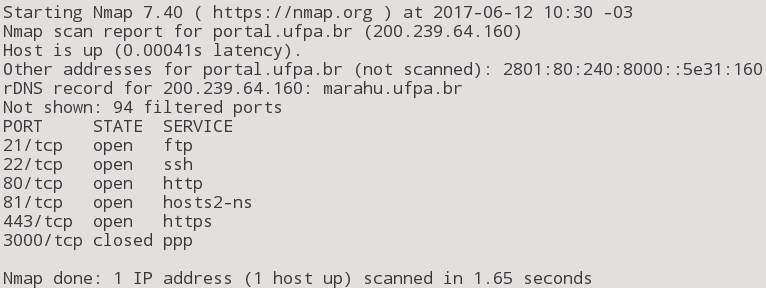
\includegraphics[scale=.5]{nmap.png}
 \caption{Exemplo de saída do Nmap}
 \label{fig:nmap}
\end{figure}

\subsection{Metasploit Framework} \label{sec:metasploit}

O Metasploit é um \textit{framework} de código aberto cujo principio básico é desenvolver e executar \textit{exploit} contra alvos remotos e fornecer uma lista de vulnerabilidades existentes no alvo. É uma ferramenta que combina diversos \textit{exploits} e payloads dentro de um local, ideal para levantamento de segurança de serviços e testes de penetração \cite{metasploit:yash}.  

O Metasploit possui uma biblioteca divida em três partes: \textbf{Rex}: É a biblioteca fundamental, a maioria das tarefas executadas pelo \textit{framework} usaram essa biblioteca; \textbf{MSF Core}: É o \textit{framework} em si, possui, por exemplo, gerenciador de módulos e a base de dados; \textbf{MSF Base}: Guarda os módulos, sejam eles, \textit{exploit}, \textit{encoders} (ferramentas usadas para desenvolver o \textit{payloads}) e os \textit{payloads}. Além disso, são guardadas informações de configuração e sessões criadas pelos \textit{exploits}. A arquitetura é mostrada com mais detalhes na figura \ref{fig:arqmetasploit}. 

Os módulos são divididos da seguinte maneira: Payload: são código executados no alvo remotamente; Exploit: explora \textit{bugs} ou vulnerabilidade existente em aplicações do alvo; Módulos Auxiliares: usado para escanear as vulnerabilidades e executar várias tarefas; Encoder: codifica o \textit{payload} para evitar qualquer tipo de detecção pelo anti vírus.

\textbf{Interface}: Disponibiliza a parte gráfica para o usuário;

\begin{figure}[!htb]
 \centering
 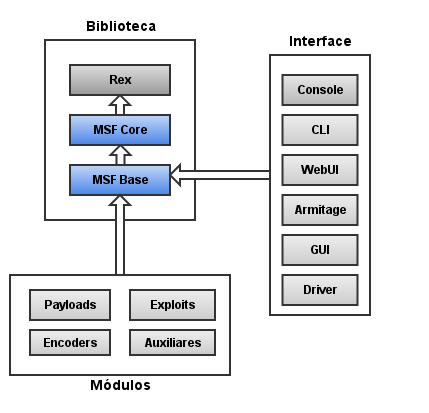
\includegraphics[scale=.6]{metasploit_arquitetura.png}
 \caption{Arquitetura do Metasploit}
 \label{fig:arqmetasploit}
\end{figure}

\subsection{Pytbull} \label{sec:pytbull}

O Pytbull é um \textit{framework} para teste de IDPS, capaz de determinar a capacidade de detecção e bloqueio do mesmo, além de fazer uma comparação entre diversas soluções e verifica as configurações \cite{pytbull}. O \textit{framework} Pytbull possui cerca de 300 testes agrupados em 11 módulos, temos:

\begin{itemize}
 \item \textbf{badTraffic}: pacotes não compatíveis com a RFC são enviados para o servidor para testar como os pacotes são processados; 
 \item \textbf{bruteForce}: testa a capacidade do IDPS de rastrear ataques de força bruta;
 \item \textbf{clientSideAttacks}: usa um \textit{shell} reverso para fornecer ao servidor instruções para baixar arquivos maliciosos; 
 \item \textbf{denialOfService}: testa a capacidade do IDPS de proteger contra tentativas de DoS; 
 \item \textbf{evasionTechniques}: testa a capacidade do IDPS de detectar técnicas de evasão; 
 \item \textbf{fragmentedPackets}: várias cargas úteis fragmentadas são enviadas ao servidor para testar sua capacidade de recomposição e detectar os ataques; 
 \item \textbf{ipReputation}: testa a capacidade do servidor detectar tráfego de servidores com reputação baixa;
 \item \textbf{normalUsage}: cargas úteis que correspondem a uso normal; 
 \item \textbf{pcapReplay}: permite reproduzir arquivos pcap; 
 \item \textbf{shellCodes}: envia \textit{shellcodes} para o servidor na porta 21/ftp testando a capacidade de detectar e/ou bloquear o mesmo; 
 \item \textbf{testRules}, testa a base de assinaturas configuradas no servidor IDPS.
\end{itemize}

Existem basicamente 5 tipos de testes: socket, abre um \textit{socket} em uma porta e envia o \textit{payload} para o alvo remoto na porta especificada; command, envia um comando para alvo remoto com a função python subprocess.call(); scapy, envia cargas úteis especificas baseadas na sintaxe de Scapy; client side attacks, usa um \textit{shell} reverso no alvo remoto e envia comandos para serem processados no servidor; pcap replay, permite reproduzir tráfego com base em arquivos de pcap.

\begin{figure}[!htb]
 \centering
 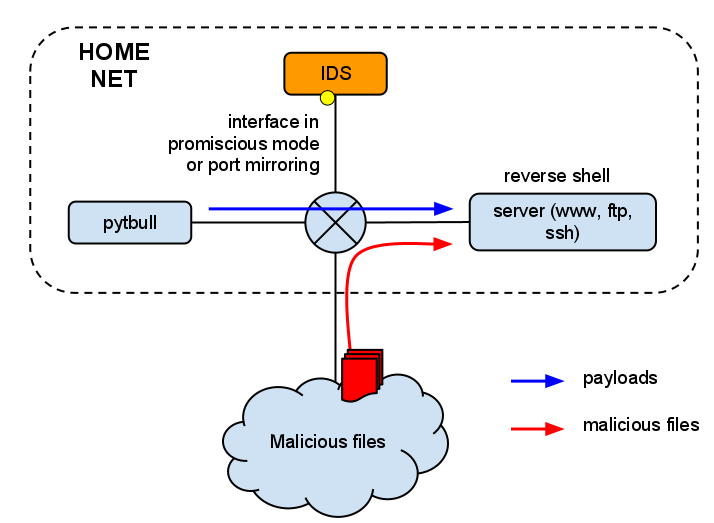
\includegraphics[scale=.4]{arquitetura_pytbull.png}
 \caption{Arquitetura do \textit{framework} Pytbull}
 \label{fig:pytbull}
\end{figure}

\
\section{Conclusão}
%Este capítulo apresentou
\chapter{Sistemas de Detecção e Prevenção de Intrusão}
%breve texto introduzindo o capítulo + apresentação das seções
\section{Definições de IDS/IPS}

\textit{Intrusion Detection Systems} (IDS) ou Sistemas de Detecção de Intrusão (SDI) são ferramentas utilizadas para monitoramento de eventos que ocorrem em redes e sistemas computacionais, analisando sinais de possíveis ataques que podem levar a uma violação das politicas de segurança da organização, alertando os administradores do sistema que estes eventos estão ocorrendo. O \textit{Intrusion Detection Systems} (IPS) ou Sistema de Prevenção de Intrusão (SPI) possui todas as funcionalidades do IDS com uma diferença, ele é capaz de deter alguns possíveis incidentes, minimizando os impactos causados por sistemas comprometidos \cite{mukhopadhyay01}.

Basicamente os sistemas de detecção de intrusão são compostos por quatro componentes, temos: Sensor ou Agente, responsável pelo monitoramento e analise do trafego capturado; Banco de Dados, usado como repositório das informações de eventos detectados pelos sensor ou agente que serão processados; Gestor, é o dispositivo central que recebe, analisa e gerencia as informações de eventos vindos do sensor ou agente; Console, fornece uma interface para administração e monitoramento das atividades do IDS.

\section{Tipos de IDS/IPS}

Os IDSs são classificados de acordo com o local onde o sensor é instalado, \textit{Host Based Intrusion Detection Systems} (HIDS) e \textit{Network Based Intrusion Detection Systems} (NIDS), e a técnica utilizada para o monitoramento, baseado em assinaturas e anomalias \cite{nagahama2012ipsflow}.

Em um HIDS o sensor é instalado no \textit{host} que será monitorado, analisando as informações contidas na própria máquina. Esse tipo de IDS tem o objetivo de analisar aspectos internos ao \textit{host} como processos em execução, modificações na configuração do sistema e serviços, monitorar o tráfego de rede somente do \textit{host} e acesso a arquivos não autorizados, entre outros.

Os HIDS possuem algumas vantagens como evitar que alguns códigos sejam executados; bloqueia o tráfego de entrada e saída contendo ataques e uso não autorizado de protocolos e programas; evita que arquivos possam ser acessados, modificados e deletados impedindo o instalação de \textit{malware} e outros ataques envolvendo acesso inapropriado a arquivos. Por outro lado, um HIDS possui algumas limitações como, por exemplo, difícil instalação e manutenção; interferir no desempenho do \textit{host}; demora para identificar alguns eventos consequentemente a resposta a esses incidentes sofrerá um \textit{delay} \cite{scarfone01}.

Já em um NIDS, o sensor é instalado na rede e a interface de rede atua em um modo especial chamado ``promíscuo'', passando a ter a capacidade de capturar o tráfego da rede mesmo que os pacotes não sejam destinados ao próprio sensor.

Quanto a localização o NIDS pode ser classificado como passivo ou ativo. No modo passivo, o IDS monitora copias dos pacotes da rede que passam pelo \textit{switch} ou \textit{hub} onde está conectado, ficando limitado somente a gerar notificações quando encontrado algum tráfego malicioso. Enquanto no modo ativo, o IDS é instalado da forma que o tráfego da rede passe através do sensor parecendo com o fluxo de dados associado com um \textit{firewall}. Dessa forma, ele é capaz de parar ataques bloqueando o fluxo malicioso (Figura \ref{nids}). 

Os NIDS possuem algumas vantagens como serem independentes de plataforma; não interfere no desempenho do \textit{host}; fácil implantação e transparente para o atacante. Por outro lado, possuem desvantagens como: pode adicionar retardados nos pacotes quando instalado no modo ativo, isso ocorre principalmente se houver um subdimensionamento do \textit{hardware}; dificuldade de tratar dados de redes de alta velocidade; quando em modo passivo, trata apenas o segmento da rede que o IDS esta instalado e dificuldade de tratar dados criptografados. Esse tipo de IDS é mais utilizado devido a grande heterogeneidade de dispositivos e sistemas operacionais disponíveis na rede, tornando a administração mais simples se comparados com o HIDS.

Quanto a técnica de monitoramento utilizado, o IDS pode ser baseados em assinaturas ou anomalias. IDSs baseados em assinaturas compara os pacotes com uma base de assinaturas de ataques previamente conhecidos e reportados por especialistas, cada assinatura identifica um ataque. Tem como vantagem, usar poucos recursos do servidor e rápido processamento. Porém, as desvantagens são: exigi uma atualização constante da base de assinaturas; alto conhecimento para geração da base e possuir um alto índice de falsos positivos e negativos.

Já os baseados em anomalias, procuram determinar um comportamento normal na fase de aprendizagem do sistema computacional ou rede e sempre que existir um desvio desse padrão alertas são gerados. Possui a vantagem de detectar novos ataques sem necessariamente conhecer a fundo a intrusão através dos desvio de comportamento. Porém existe a desvantagem de gerar um grande número de falsos alertas em decorrência a modificações na rede ou \textit{host} nem sempre representar um tráfego malicioso. 

\begin{figure}[!htb]
 \centering
  \subfloat[NIDS Passivo]{
    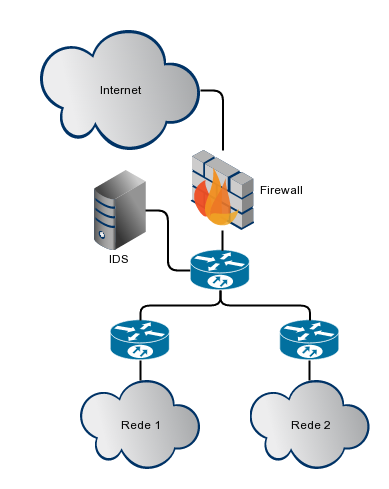
\includegraphics[height=7cm]{nids_passivo.png}
    \label{nids-passivo}
  }
  \quad
  \subfloat[NIDS Ativo]{
    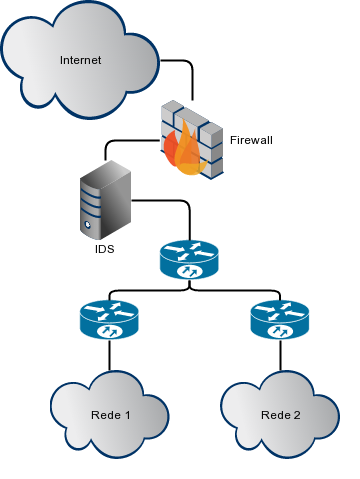
\includegraphics[height=7cm]{nids_ativo.png}
    \label{nids-ativo}
  }
  \caption{Exemplos de Arquitetura de NIDS}
  \label{nids}
 \end{figure}

\section{Principais Ferramentas de IDS}
\subsection{Snort}

O Snort é um sistema de detecção e prevenção de intrusão de código fonte aberto escrita na linguagem de programação C bem conhecido pela comunidade da segurança da informação. Seu primeiro \textit{release} foi lançado em 1998 e desde então passa por constantes revisões e aperfeiçoamentos, com o passar dos anos se tornou o IDS mais utilizado no mundo. Ele combina análise baseada em assinaturas e anomalias, podendo operar em três modos: \textit{sniffer}, \textit{packet logger} e de sistema de detecção de intrusão (NIDS) \cite{snortorgbr}.

No modo \textit{Sniffer}, o Snort captura os pacotes e exibi as informações no console. No modo \textit{Packet Logger}, além de capturar o tráfego, ele registrar essas informações em disco (arquivos de logs). E no modo NIDS, é o modo mais complexo, permite analise do pacotes de rede em tempo real.

Existe quatro componentes no Snort: O \textit{Sniffer}, o Pré-processador, o Motor de Detecção e Módulo de Saída. Os componentes são organizados de acordo com a figura \ref{snort-componentes} \cite{kohlenberg2007snort}.

\begin{figure}[!htb]
  \centering
  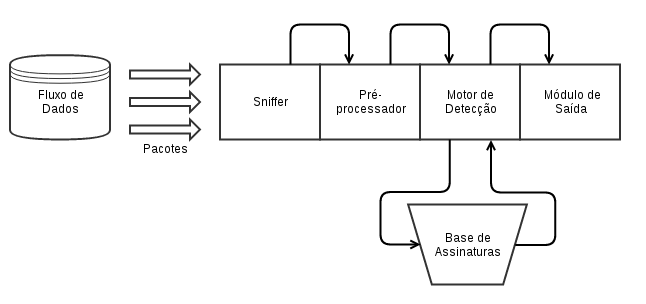
\includegraphics[scale=0.6]{snort_componentes}
  \caption{Componentes do Snort}
  \label{snort-componentes}
\end{figure}

\subsection{Suricata}
\section{Conclusão}
%Ex: Este capítulo apresentou...

\chapter{Detecção de Intrusão em um Cenário Real}
%- Em cada capitulo adicionar um texto introdutório

Este capítulo esta organizado da seguinte forma: A próxima seção apresenta o cenário de testes, descrevendo características gerais da rede selecionada para os teste. Na seção \ref{sec:infraestrutura} será abordado a infraestrutura usada para os testes, ferramentas utilizadas e as configurações feitas. Na seção \ref{sec:testes} será descrito os testes realizados com suas respectivas justificativas. Na seção \ref{sec:resultados} será apresentado os resultados esperados e obtidos, problemas encontrados e a comparação das ferramentas e por último, na seção \ref{sec:conclusão}, uma breve conclusão.

\section{Metodologia dos Testes}
% (Adicionar o escopo dos testes): descrever o ambientes,
\subsection{Cenário de Testes} \label{sec:cenário}
%Descrever o cenário. Ex: Uma rede com XXX usuários; Os usuários utilizam
%diferentes ferramentas,...
%Adicionar gráficos de utilização da rede

A rede selecionada para ser monitorada tem os valores especificados na tabela. Podemos verificar que em um determinado período do dia o pico de trafego chega a 107,25 Mbps, valores considerados ideais para o experimento, inclusive para tentar validar os recursos alocados. Figura \ref{fig:ilc}

Em um primeiro momento, selecionou-se uma rede

\subsection{Infraestrutura Definida para Testes} \label{sec:infraestrutura}
%Descrever o que foi utilizado:
%Ex: Equipamentos - Servidores, ....
%    Configuração
%    Ferramentas - Snort (referenciar capítulo), ...

No ambiente de teste foi usado uma máquina Dell com 134 Megabytes (MB) de memória RAM e 40 núcleos. Usou-se XenServer \cite{xenserver} versão 7, sistema operacional (SO) \textit{opensource} da Citrix voltado para virtualização. Foram testados outros SOs porém somente o XenServer possuía, na época da instalação do ambiente, \textit{firmware} da placa de rede do \textit{host} compatível e que funcionava com instabilidade. Outro fator que pesou na escolha do SO foi a experiência que tinha com a plataforma e por existir uma interface para gerencia chamada XenCenter que roda no Windows. Uma alternativa \textit{opensource} desse software é o OpenXenManager \cite{openxenmanager}.

No primeiro momento, foi instalado uma máquina virtual com o sistema operacional Debian 7.11 \textit{codename} Wheezy \cite{debianwheezy}, uma distribuição linux com uma proposta de ser totalmente livre, usada como base para instalação de outras máquinas utilizando o recurso de \textit{snapshot}, uma cópia de uma máquina virtual rodando em um certo momento, do XenServer. O uso desse recurso foi necessário para criar um ambiente igual para os IDSs.

Foi alocado 8 MB memória RAM, 4 processadores e 100 Gigabytes(GB) de espaço em disco para o \textit{snapshot}. Esses valores foram definidos com base em um estudo \cite{mikelococo} que considerava vários fatores, como largura da rede, localização do IDS e versão, tipo do capturador de tráfego e tamanho da base de assinaturas para dimensionar os recursos de memória e processamento, aplicado especificamente ao Snort. A mesma regra foi aplicada ao Suricata.

Para o \textit{host} conseguir pegar o pacotes destinados a rede escolhida para ser monitorada foi necessário uma configuração de espelhamento no roteador B (Figura \ref{fig:infra-ambiente}) que consiste na copia dos pacotes que saem pela porta dessa rede no roteador para a porta conectada no \textit{host} que possui uma largura de banda de 10 Gigabits. A interface de rede do \textit{host} precisou ser configurada no modo \textit{promisc}.

Posteriormente criou-se três máquinas virtuais, duas usadas para instalação dos IDSs (Suricata e Snort) e a terceira para instalação das ferramentas usadas para simular ataques a rede. Optou-se pela instalação do sistema Kali Linux \cite{kalilinux} para geração de ataques pois nele existe várias ferramentas nativas para testes de penetração e auditoria de segurança. A infraestrutura final pode ser visualizada na Figura \ref{fig:infra-ambiente}.

\begin{figure}[!htb]
 \centering
 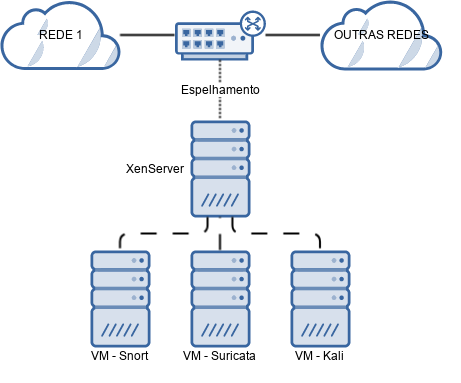
\includegraphics[scale=.5]{infra.png}
 \caption{Infraestrutura do ambiente de teste}
 \label{fig:infra-ambiente}
\end{figure}

Para coleta das informações de uso de recurso de hardware como memória, processamento e I/O das máquinas com os IDSs foi usado o \textit{daemon} Collectd \cite{collectd}. Outra opção para esse fim é a utilização de um servidor de monitoramento com o Zabbix \cite{zabbix}. A ideia de usar duas ferramentas para analise é fazer um comparativo e validar as informações coletadas.

O formato usado para facilitar a análise do \textit{logs} foi JavaScript Object Notation (JSON), um formato simples, leve e de fácil leitura. O Motor de Saída do Suricata já tem suporte a esse tipo de formato o que não acontece no Snort. Para tal, usou-se o IDSTools \cite{py-idstools}, uma coleção de bibliotecas na linguagem python que trabalha para auxiliar o IDS, compatível com as ferramentas estudas. Dentre os utilitários presentes nessa coleção, temos o idstools-u2json, que converte, de forma continua, arquivo no formato unified2, uma das saídas disponível no Snort, para o formato JSON.

Para analisar os \textit{logs}, usou-se uma infraestrutura que combina três ferramentas, o Kibana \cite{kibana}, uma plataforma de análise e visualização desenhada para trabalhar com os índices do Elasticsearch \cite{elasticsearch}, a grosso modo, podemos dizer que ela é uma interface gráfica para o Elasticsearch. O Elasticsearch, um motor de busca e análise altamente escalável, capaz de armazenar, buscar e analisar uma grande quantidade de dados em tempo próximo ao real. Por ultimo, o Logstach \cite{logstach}, um motor de coleta de dados em tempo real, unificando os dados de diferentes fontes dinamicamente, normalizando-os nos destinos escolhidos (Figura \ref{fig:logstach}). Dessa forma centralizou-se os \textit{logs}, facilitando a visualização das ocorrências dos IDSs. 

\begin{figure}[!htb]
 \centering
 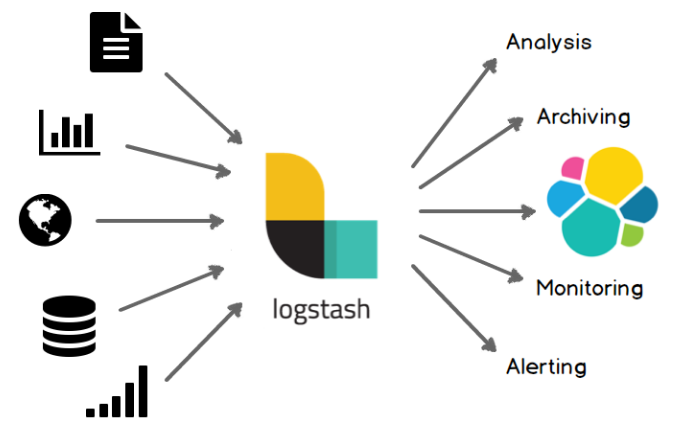
\includegraphics[scale=.4]{logstach.png}
 \caption{Busca e união dos dados de diferentes fontes}
 \label{fig:logstach}
\end{figure}
section{Testes Realizados} \label{sec:testes}
%Quais os testes realizados com justificativa ?
%Descrição dos testes. Quais os testes foram realizados ?
Os testes realizados são simulações de passos que uma pessoa má intencionada iria tomar para alguma tentativa de invasão, entende-se por invasão, qualquer tipo de violação e alteração não autorizada de um serviço ou \textit{host}.

O passo inicial seria um estudo do alvo por engenharia social, analisando as pessoas que trabalharam no organização, enviando spam e phishing na tentativa de capturar dados como senhas de acesso. Posteriormente, verificando os serviços que o alvo oferece e observando (\textit{sniffando}) a rede, a procura de alguma senha desprotegida (não criptografada). Esse passo inicial não será aplicados nos testes pois seria impossível o IDS detectar.

O passo seguinte seria um estudo e mapeamento da rede, a procura de um \textit{host} vulnerável. A ferramenta escolhida para essa finalidade é o Nmap \ref{sec:nmap}. No primeiro teste de Scan, usou-se o parâmetro "-F", habilitando a modo \textit{fast} do Nmap. Nesse modo, são verificadas apenas a portas especificadas no arquivo nmap-services, na instalação padrão esse arquivo vem com 27372 portas descritas. Isso é muito mais rápido que verificar todas as 65535 portas possíveis em um \textit{host}.

nmap -F 200.239.82.0/24

O segundo teste, usou-se o parâmetro '-sV' do Nmap. Essa opção habilita a descoberta de versões, tentando determinar os protocolos de serviços, o nome da aplicação, o número da versão, o nome do \textit{host}, tipo de dispositivo, sistema operacional usado, entre outras informações. Essas informações são de grande valor pois, a partir delas, pode-se explorar vulnerabilidades conhecidas de uma determinada versão de um serviço \cite{nmap}.

nmap -sV 200.239.82.0/24

De posse de um alvo em potencial, próximo passo seria rodar um scan de vulnerabilidade, em busca de brejas já conhecidas, e que, geralmente por descuido do administrador, não foi fechada. Para esses testes usou-se o \textit{framework} Metasploit \ref{sec:metasploit} nativo do sistema operacional Kali Linux.

\section{Resultados} \label{sec:resultados}
%Resultados esperados e obtidos
%Quais os resultados dos testes ??
%Comparação das ferramentas
%Problemas encontrados
\section{Conclusão} \label{sec:conclusão}
\section{Métricas de Comparação}
%Consumo dos Recursos de Hardware (Memória, Processamento)
%Taxa de Detecção
%Número de Falsos Positivos/Negativos
\chapter{Considerações Finais e Trabalhos Futuros} \label{considerações}
\phantompart
\postextual
\bibliography{bib/dissertacao}
\phantompart
\printindex
\end{document}
